\documentclass[12pt]{article}

\usepackage[margin=1in]{geometry}
\usepackage[T1]{fontenc}
\usepackage{lmodern}
\usepackage{microtype}
\usepackage{amsmath,amssymb,mathtools}
\usepackage{booktabs}
\usepackage{enumitem}
\usepackage{setspace}
\usepackage{xcolor}
\usepackage{tikz}
\usepackage{hyperref}
\usepackage{xurl}

\hypersetup{
  colorlinks=true,
  linkcolor=black,
  citecolor=black,
  urlcolor=blue,
  pdftitle={The Magnetic Slope: From Dipole Interaction Energy to Translational Acceleration},
  pdfauthor={Light-Meter Physics},
  pdfsubject={Magnetic dipole energy gradients, frequency normalization, and acceleration},
  pdfkeywords={magnetic dipole, interaction energy, force gradient, frequency equivalent, acceleration}
}

\onehalfspacing
\widowpenalty=10000
\clubpenalty=10000
\definecolor{ink}{HTML}{172E3D}
\definecolor{teal}{HTML}{126D77}
\definecolor{rust}{HTML}{B1533E}

\title{The Magnetic Slope:\\
From Dipole Interaction Energy to Translational Acceleration}
\author{Light-Meter Physics}
\date{}

\begin{document}

\maketitle

\begin{abstract}
A magnetic field's local strength does not, by itself, determine the translational force on a magnetic dipole; the spatial change of its interaction energy matters. For a localized permanent dipole with fixed moment in a static external field, this manuscript starts from $U_{\rm mag}=-\boldsymbol{\mu}\cdot\mathbf B$ and the corresponding force gradient. It then expresses the signed interaction energy in frequency units, normalizes it by the same body's rest energy, and derives the low-speed relation $\mathbf a_{\rm mag}=c^2\nabla\epsilon_{\rm mag}$. A one-dimensional aligned model makes the role of the field gradient explicit. An illustrative comparison uses an assumed magnetic slope of $2.45\times10^{-13}\,\mathrm{m^{-1}}$ and an Earth-surface standard-gravity benchmark; a separate inverse calculation estimates the field gradient required for an assumed dipole. These numerical inputs are examples, not measurements or specifications for a particular magnet. The frequency equivalent is an energy normalization, not by itself an oscillator or a literal clock rate. The construction is a rewriting of standard dipole energetics within stated assumptions, not a universal gravitational law or a new force mechanism.
\end{abstract}

\noindent\textbf{Keywords:} magnetic dipole, interaction energy, force gradient, frequency equivalent, rest-energy normalization, acceleration

\section{Introduction}

A magnetic field can be strong and still exert no net translational force on an aligned permanent dipole if the field is uniform over the dipole's motion. Conversely, a spatial gradient can produce a force even when the field's value at a chosen point is the same. The distinction is between field strength and the slope of the interaction energy.

This manuscript develops that distinction using a deliberately limited model. A small permanent magnetic dipole has fixed moment $\boldsymbol{\mu}$ and fixed mass $m$. It moves slowly through a static external magnetic field whose variation across the dipole is small enough for the point-dipole approximation. The derivation is translational and nonrelativistic. Induced or hysteretic magnetic materials, detailed apparatus designs, and relativistic motion are outside its scope.

The term \emph{magnetic slope} will refer to the spatial gradient of a dimensionless magnetic interaction-energy ratio. The sequence is
\begin{equation}
  U_{\rm mag}=-\boldsymbol{\mu}\cdot\mathbf B,
  \qquad
  \nu_{\rm mag}=-\frac{U_{\rm mag}}{h},
  \qquad
  \epsilon_{\rm mag}=\frac{\nu_{\rm mag}}{\nu_C}
                   =-\frac{U_{\rm mag}}{mc^2},
  \qquad
  \mathbf a_{\rm mag}=c^2\nabla\epsilon_{\rm mag}.
  \label{eq:argument-chain}
\end{equation}
The frequency and rest-energy steps are unit conversions and normalizations. They do not add a new magnetic law. The physical claims below are those of the fixed-dipole model under the assumptions stated here.

\section{Model, assumptions, and notation}
\label{sec:model}

Let $\mathbf B(\mathbf x)$ be a time-independent magnetic flux density produced externally. The dipole is localized near its center-of-mass position $\mathbf x$, has a fixed magnetic moment $\boldsymbol{\mu}$, and has constant inertial mass $m$. Its characteristic size is assumed small compared with the length scale on which the external field changes. In using the standard compact force formula, the local field is taken to satisfy the assumptions of the point-dipole derivation; in particular, the field is static and curl-free in the dipole's neighborhood. The usual derivation also separates the net force on the center of mass from the torque that changes orientation \cite{TongDipole}.

The translational equation of motion is Newtonian,
\begin{equation}
  m\mathbf a=\mathbf F,
  \label{eq:newtonian-motion}
\end{equation}
so the speed remains small compared with $c$ over the regime being described. Here $\mathbf a$ is acceleration measured in the chosen laboratory frame. This assumption is essential to the simple relation derived later; that relation is not asserted as a relativistic equation of motion.

The symbols and units used throughout are summarized below.
\begin{center}
\small
\begin{tabular}{@{}lll@{}}
  \toprule
  Symbol & Meaning & SI unit \\
  \midrule
  $m$ & fixed inertial mass & $\mathrm{kg}$ \\
  $\boldsymbol{\mu}$ & magnetic dipole moment & $\mathrm{A\,m^2}$ \\
  $\mathbf B$ & external magnetic flux density & $\mathrm T$ \\
  $U_{\rm mag}$ & magnetic interaction potential energy & $\mathrm J$ \\
  $\nu_{\rm mag}$ & signed frequency equivalent of $-U_{\rm mag}$ & $\mathrm{Hz}$ \\
  $\nu_C$ & rest-energy frequency scale $mc^2/h$ & $\mathrm{Hz}$ \\
  $\epsilon_{\rm mag}$ & normalized interaction-energy ratio & dimensionless \\
  \bottomrule
\end{tabular}
\end{center}

\section{Interaction energy and translational force}
\label{sec:energy-force}

For a fixed magnetic moment in a static external field, the magnetic interaction energy is
\begin{equation}
  U_{\rm mag}(\mathbf x)
  =-\boldsymbol{\mu}\cdot\mathbf B(\mathbf x).
  \label{eq:dipole-energy}
\end{equation}
The translational force is the negative spatial gradient of the potential:
\begin{equation}
  \mathbf F=-\nabla U_{\rm mag}
  =\nabla\!\left(\boldsymbol{\mu}\cdot\mathbf B\right),
  \label{eq:dipole-force}
\end{equation}
where the gradient is taken at fixed $\boldsymbol{\mu}$. The force expression applies under the local dipole assumptions stated in Sec.~\ref{sec:model}; it is not a general constitutive law for every magnetic material \cite{TongDipole}.

The dipole can also experience a torque,
\begin{equation}
  \boldsymbol{\tau}_{\rm mag}
  =\boldsymbol{\mu}\times\mathbf B.
  \label{eq:dipole-torque}
\end{equation}
A uniform field therefore can exert a torque on a misaligned dipole without exerting a translational force in this idealized model. The fixed-vector approximation assumes constrained orientation, or an aligned axial trajectory along which the torque vanishes; it focuses on translation and does not model alignment dynamics.

For motion along a selected axis $x$, define the signed field component along the fixed dipole direction by
\begin{equation}
  B_{\parallel}(x)
  \equiv\widehat{\boldsymbol{\mu}}\cdot\mathbf B(\mathbf x(x)),
  \qquad
  \mu\equiv|\boldsymbol{\mu}|.
  \label{eq:parallel-field}
\end{equation}
In the aligned one-dimensional example, $U_{\rm mag}=-\mu B_{\parallel}(x)$ and
\begin{equation}
  F_x=-\frac{dU_{\rm mag}}{dx}
     =\mu\frac{dB_{\parallel}}{dx}.
  \label{eq:one-dimensional-force}
\end{equation}
Thus a positive field-component gradient gives a force toward $+x$ for $\mu>0$ aligned with the field. The scalar function $B_{\parallel}(x)$ describes the field sampled along the path; it is not a claim that a globally one-dimensional vector field $\mathbf B=(B(x),0,0)$ is a physical field configuration.

\begin{figure}[ht]
  \centering
  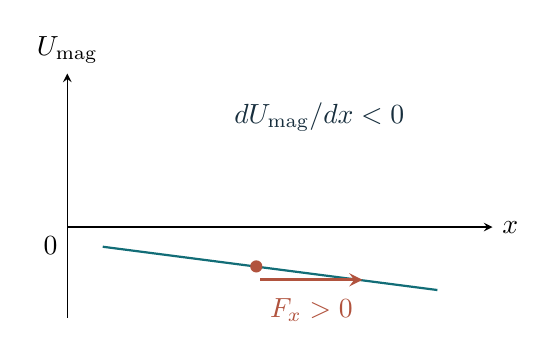
\begin{tikzpicture}[x=1cm,y=1cm,>=stealth]
    \draw[->] (0,1.15)--(5.4,1.15) node[right] {$x$};
    \draw[->] (0,0)--(0,3.1) node[above] {$U_{\rm mag}$};
    \draw[thick,teal] (0.45,0.9)--(4.7,0.35);
    \fill[rust] (2.4,0.65) circle (2.2pt);
    \draw[rust,->,line width=1.1pt] (2.45,0.48)--(3.75,0.48)
      node[midway,below=3pt] {$F_x>0$};
    \node[below left] at (0,1.15) {$0$};
    \node[ink] at (3.2,2.55) {$dU_{\rm mag}/dx<0$};
  \end{tikzpicture}
  \caption{Schematic potential-energy profile for an aligned dipole moving along $+x$. The horizontal axis marks $U_{\rm mag}=0$; the plotted values are negative, consistent with $U_{\rm mag}=-\mu B_{\parallel}$ for an aligned positive field. A negative slope corresponds to a positive translational force $F_x=-dU_{\rm mag}/dx$. The drawing is illustrative, not a measured field or apparatus profile.}
  \label{fig:potential-slope}
\end{figure}

\section{Field strength and field slope}
\label{sec:field-slope}

Equation~\eqref{eq:one-dimensional-force} depends on the spatial derivative of the field component, not merely its value at one position. A uniform profile has $dB_{\parallel}/dx=0$ and therefore $F_x=0$ for the aligned fixed dipole. An increasing profile has $dB_{\parallel}/dx>0$ and produces $F_x>0$ under the same alignment assumption.

\begin{figure}[ht]
  \centering
  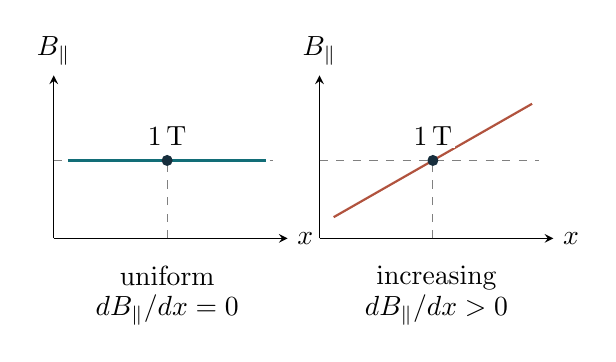
\begin{tikzpicture}[x=0.9cm,y=0.9cm,>=stealth]
    \draw[->] (0.25,0.35)--(3.55,0.35) node[right] {$x$};
    \draw[->] (0.25,0.35)--(0.25,2.65) node[above] {$B_{\parallel}$};
    \draw[dashed,gray] (0.25,1.45)--(3.35,1.45);
    \draw[thick,teal] (0.45,1.45)--(3.25,1.45);
    \draw[dashed,gray] (1.85,0.35)--(1.85,1.45);
    \fill[ink] (1.85,1.45) circle (2pt);
    \node[fill=white,inner sep=1pt] at (1.85,1.8) {$1\,\mathrm T$};
    \node[anchor=north] at (1.85,0.1) {uniform};
    \node[anchor=north,align=center] at (1.85,-0.3) {$dB_{\parallel}/dx=0$};

    \draw[->] (4.0,0.35)--(7.3,0.35) node[right] {$x$};
    \draw[->] (4.0,0.35)--(4.0,2.65) node[above] {$B_{\parallel}$};
    \draw[dashed,gray] (4.0,1.45)--(7.1,1.45);
    \draw[thick,rust] (4.2,0.65)--(7.0,2.25);
    \draw[dashed,gray] (5.6,0.35)--(5.6,1.45);
    \fill[ink] (5.6,1.45) circle (2pt);
    \node[fill=white,inner sep=1pt] at (5.6,1.8) {$1\,\mathrm T$};
    \node[anchor=north] at (5.65,0.1) {increasing};
    \node[anchor=north,align=center] at (5.65,-0.3) {$dB_{\parallel}/dx>0$};
  \end{tikzpicture}
  \caption{Two schematic axial profiles have the same local field component, $B_{\parallel}=1\,\mathrm T$, but different derivatives. The local value alone does not determine the translational force. Profiles represent the field sampled along a path, not a complete three-dimensional field map.}
  \label{fig:field-value-gradient}
\end{figure}

A uniform field can still exert torque if the dipole is misaligned, as Eq.~\eqref{eq:dipole-torque} shows. The comparison in Fig.~\ref{fig:field-value-gradient} concerns translational force for an aligned dipole. Its $1\,\mathrm T$ labels are illustrative local field values; they do not specify a magnetic moment or a field gradient.

\section{Energy expressed in frequency units}
\label{sec:frequency}

Planck's constant converts energy to ordinary frequency units. Define the signed magnetic frequency equivalent by
\begin{equation}
  \nu_{\rm mag}
  \equiv-\frac{U_{\rm mag}}{h}
  =\frac{\boldsymbol{\mu}\cdot\mathbf B}{h},
  \qquad
  h\nu_{\rm mag}=-U_{\rm mag}.
  \label{eq:mag-frequency}
\end{equation}
Because $1\,\mathrm{J}/h$ has units of hertz, $\nu_{\rm mag}$ expresses the interaction energy on a frequency scale. For the aligned case with the zero chosen at $B_{\parallel}=0$, increasing positive $B_{\parallel}$ makes $U_{\rm mag}$ more negative and $\nu_{\rm mag}$ more positive.

An alternative signed energy-frequency convention is $\widetilde{\nu}_{\rm mag}\equiv U_{\rm mag}/h=-\nu_{\rm mag}$. Either convention gives the same force when the accompanying gradient sign is changed consistently:
\begin{equation}
  \mathbf a_{\rm mag}
  =c^2\nabla\!\left(\frac{\nu_{\rm mag}}{\nu_C}\right)
  =-c^2\nabla\!\left(\frac{\widetilde{\nu}_{\rm mag}}{\nu_C}\right).
  \label{eq:frequency-sign-conventions}
\end{equation}

The word \emph{frequency} here describes an energy equivalent; it does not assert that the dipole is oscillating. The quantity is not automatically a Larmor frequency, a transition frequency, or the rate of a physical clock. Those interpretations require a specified dynamical system and measurement model. Adding a position-independent constant to $U_{\rm mag}$ shifts $\nu_{\rm mag}$ by a constant but leaves the force, which depends on its spatial gradient, unchanged.

\section{Normalize by the rest-energy scale}
\label{sec:normalization}

For the same body's fixed mass $m$, define the rest-energy frequency scale
\begin{equation}
  \nu_C\equiv\frac{mc^2}{h}.
  \label{eq:rest-frequency}
\end{equation}
This is a normalization scale. In particular, using it for a macroscopic dipole does not claim that the body is an observed Compton clock. The ratio
\begin{equation}
  \epsilon_{\rm mag}
  \equiv\frac{\nu_{\rm mag}}{\nu_C}
  =-\frac{U_{\rm mag}}{mc^2}
  =\frac{\boldsymbol{\mu}\cdot\mathbf B}{mc^2}
  \label{eq:energy-ratio}
\end{equation}
is dimensionless. It compares the magnetic interaction energy, with the sign convention of Eq.~\eqref{eq:mag-frequency}, with the body's rest energy. The sign of $\epsilon_{\rm mag}$ depends on orientation and the chosen energy reference; the aligned examples take $\boldsymbol{\mu}\cdot\mathbf B>0$.

\section{Derivation of the magnetic slope}
\label{sec:derive-slope}

Combining the Newtonian equation of motion with the potential-energy force gives
\begin{equation}
  m\mathbf a
  =\mathbf F
  =-\nabla U_{\rm mag}
  =h\nabla\nu_{\rm mag}.
  \label{eq:force-frequency}
\end{equation}
Since $m$ is fixed, Eq.~\eqref{eq:rest-frequency} implies
\begin{equation}
  \frac{h}{m}=\frac{c^2}{\nu_C}.
  \label{eq:h-over-m}
\end{equation}
Dividing Eq.~\eqref{eq:force-frequency} by $m$ and using Eq.~\eqref{eq:energy-ratio} yields
\begin{equation}
  \mathbf a_{\rm mag}
  =\frac{h}{m}\nabla\nu_{\rm mag}
  =c^2\nabla\!\left(\frac{\nu_{\rm mag}}{\nu_C}\right)
  =c^2\nabla\epsilon_{\rm mag}.
  \label{eq:mag-acceleration}
\end{equation}
The units are consistent: $\nabla\epsilon_{\rm mag}$ has units of inverse length, so multiplication by $c^2$ gives acceleration. Equation~\eqref{eq:mag-acceleration} is not an independent law; it follows from the force law, the stated frequency definition, constant mass, and the nonrelativistic equation $m\mathbf a=\mathbf F$.

In the aligned one-dimensional model,
\begin{equation}
  a_x=\frac{\mu}{m}\frac{dB_{\parallel}}{dx},
  \qquad
  \frac{a_x}{c^2}=\frac{d\epsilon_{\rm mag}}{dx}
    =\frac{\mu}{mc^2}\frac{dB_{\parallel}}{dx}.
  \label{eq:one-dimensional-acceleration}
\end{equation}
We define the signed slope along $x$ as $s_x\equiv a_x/c^2=d\epsilon_{\rm mag}/dx$. When comparing magnitudes, write
\begin{equation}
  s\equiv\frac{|a|}{c^2},
  \label{eq:slope-magnitude}
\end{equation}
which has units of $\mathrm{m^{-1}}$. For the aligned dipole, this magnitude depends on $\mu/m$ and on the local field gradient. It is therefore material- and orientation-dependent, not a universal property of a magnetic field or a gravitational lapse.

\section{A one-centimetre light-time comparison}
\label{sec:length-time}

A distance $L$ can also be represented by its vacuum light-crossing time,
\begin{equation}
  T_L\equiv\frac{L}{c}.
  \label{eq:light-time}
\end{equation}
Here $L=x_2-x_1>0$ is a center-of-mass displacement interval, not a specified diameter or length of the dipole. The dipole's dimensions must independently satisfy the small-dipole assumption in Sec.~\ref{sec:model}. Within the fixed-mass model, integrating the one-dimensional relation gives the exact endpoint identity
\begin{equation}
  \Delta\epsilon_{\rm mag}
  \equiv\epsilon_{\rm mag}(x_2)-\epsilon_{\rm mag}(x_1)
  =\frac{1}{c^2}\int_{x_1}^{x_2}a_x(x)\,\mathrm dx
  =-\frac{U_{\rm mag}(x_2)-U_{\rm mag}(x_1)}{mc^2}.
  \label{eq:epsilon-integral}
\end{equation}
If $a_x$ is nearly constant and positive over the interval, this reduces to
\begin{equation}
  \Delta\epsilon_{\rm mag}
  \simeq\frac{a_x}{c^2}L
  =\frac{a_x}{c}T_L.
  \label{eq:epsilon-distance}
\end{equation}
For the assumed slope $s_{\rm mag}=2.45\times10^{-13}\,\mathrm{m^{-1}}$ and interval $L=0.01\,\mathrm m$,
\begin{equation}
  T_L\simeq33.36\,\mathrm{ps},
  \qquad
  \Delta\epsilon_{\rm mag}\simeq s_{\rm mag}L
     =2.45\times10^{-15}.
  \label{eq:one-centimetre-example}
\end{equation}
This rewrites a spatial energy-ratio difference using light-time units. $T_L$ is not the dipole's mechanical response time, an oscillation period, or a relaxation time. Nor does a gradient measured at one point establish that the gradient remains constant over a full centimetre.

\section{Comparison with a standard-gravity benchmark}
\label{sec:comparison}

Acceleration magnitudes can be expressed using the common inverse-length scale $s=|a|/c^2$. For the Earth comparison, use conventional standard gravity $g_n=9.80665\,\mathrm{m\,s^{-2}}$ as a benchmark, not as a site-specific measurement \cite{JCGM}. The magnetic slope below is an illustrative assumed input. With the exact SI values of $c$ and $h$ used for the conversions \cite{BIPM},
\begin{align}
  s_{\rm Earth}&\equiv\frac{g_n}{c^2}
     \simeq1.0911\times10^{-16}\,\mathrm{m^{-1}},\\
  s_{\rm mag}&\equiv2.45\times10^{-13}\,\mathrm{m^{-1}},\\
  a_{\rm mag}&=c^2s_{\rm mag}
     \simeq2.20\times10^4\,\mathrm{m\,s^{-2}},\\
  \frac{s_{\rm mag}}{s_{\rm Earth}}&\simeq2.25\times10^3.
  \label{eq:slope-comparison-values}
\end{align}
The ratio compares magnitudes in a shared unit convention. It does not make magnetic and gravitational forces physically equivalent, nor does it identify a magnetic slope with a gravitational clock-rate field.

\begin{table}[ht]
  \centering
  \small
  \begin{tabular}{@{}lccp{6.2cm}@{}}
    \toprule
    Case & $s=|a|/c^2$ ($\mathrm{m^{-1}}$) & $|a|$ ($\mathrm{m\,s^{-2}}$) & Status \\
    \midrule
    Earth benchmark & $1.09\times10^{-16}$ & $9.81$ & Standard-gravity value used as a reference \\
    Magnetic example & $2.45\times10^{-13}$ & $2.20\times10^4$ & Assumed slope; acceleration inferred from $c^2s$ \\
    \bottomrule
  \end{tabular}
  \caption{Acceleration scales expressed per unit length. The magnetic slope is an illustrative input, not a measured field property. Values are rounded.}
  \label{tab:slope-comparison}
\end{table}

\section{What would the assumed slope require?}
\label{sec:inverse-example}

An inverse calculation translates the assumed acceleration into a force and a local field gradient for a chosen dipole. Take
\begin{equation}
  m=0.001\,\mathrm{kg},
  \qquad
  \mu=0.10\,\mathrm{A\,m^2},
  \qquad
  a_x\simeq2.20\times10^4\,\mathrm{m\,s^{-2}}.
  \label{eq:assumed-dipole-values}
\end{equation}
Then, in the aligned fixed-moment model,
\begin{align}
  F_x=ma_x&\simeq22.0\,\mathrm N,\\
  \frac{dB_{\parallel}}{dx}
  =\frac{F_x}{\mu}&\simeq220\,\mathrm{T\,m^{-1}}.
  \label{eq:inverse-gradient}
\end{align}
These are outputs conditional on the assumed $m$, $\mu$, and $s_{\rm mag}$. They do not identify a magnet product, describe a realizable apparatus, or specify how long a force acts. A field value such as $1\,\mathrm T$ does not by itself supply the required gradient or determine the dipole moment.

\begin{table}[ht]
  \centering
  \small
  \begin{tabular}{@{}lll@{}}
    \toprule
    Quantity & Value & Role in the example \\
    \midrule
    $m$ & $0.001\,\mathrm{kg}$ & Assumed body mass \\
    $\mu$ & $0.10\,\mathrm{A\,m^2}$ & Assumed fixed magnetic moment \\
    $s_{\rm mag}$ & $2.45\times10^{-13}\,\mathrm{m^{-1}}$ & Assumed slope \\
    $a_x$ & $2.20\times10^4\,\mathrm{m\,s^{-2}}$ & Inferred acceleration \\
    $F_x$ & $22.0\,\mathrm N$ & Inferred force \\
    $dB_{\parallel}/dx$ & $220\,\mathrm{T\,m^{-1}}$ & Inferred local gradient \\
    \bottomrule
  \end{tabular}
  \caption{Assumed inputs and derived quantities for the illustrative permanent-dipole example. Rounding is applied only to displayed values.}
  \label{tab:inverse-example}
\end{table}

\section{Interpretive limits}
\label{sec:limits}

The equations support a concise but limited conclusion: within the fixed-moment, static-field, point-dipole, and low-speed assumptions, a gradient of magnetic interaction energy produces translational acceleration. Their interpretation should not exceed those assumptions:
\begin{itemize}[leftmargin=*]
  \item The model treats a permanent dipole with fixed $\boldsymbol{\mu}$. An induced or hysteretic moment requires its field dependence and material response to be included in the energy and force calculation.
  \item The field varies slowly across the dipole. The plotted profiles are schematic axial samples of an external three-dimensional field, not complete field maps or proposed magnet geometries.
  \item The translational dynamics use $m\mathbf a=\mathbf F$ and constant mass. No relativistic acceleration law or high-speed trajectory is derived.
  \item The frequency $\nu_{\rm mag}$ is a signed energy equivalent, not automatically a physical oscillator frequency, transition frequency, or operational clock rate.
  \item The numerical magnetic slope, mass, moment, and length are illustrative assumptions. The field-gradient calculation is conditional on them and is not an experimental result.
  \item The scale $s=|a|/c^2$ permits a numerical comparison with standard gravity; it does not identify the magnetic force with gravity or define a universal lapse.
  \item The calculation determines neither the source apparatus's energy cost nor a force-duration history. Those require a model of the field source and the body's dynamics.
\end{itemize}

\section{Conclusion}

For a fixed magnetic dipole in a static external field, the interaction energy is $U_{\rm mag}=-\boldsymbol{\mu}\cdot\mathbf B$ and the translational force is its negative spatial gradient. In the aligned one-dimensional example this gives $F_x=\mu\,dB_{\parallel}/dx$: the gradient, rather than the local field value alone, controls the translational force.

Dividing the negative interaction energy by $h$ expresses it in frequency units; dividing by $mc^2/h$ gives the dimensionless ratio $\epsilon_{\rm mag}=-U_{\rm mag}/(mc^2)$. Under the stated Newtonian assumptions, its gradient obeys $\mathbf a_{\rm mag}=c^2\nabla\epsilon_{\rm mag}$. This is a standard force-and-energy identity in normalized form. The magnetic example and its comparison with standard gravity are pedagogical scale illustrations, not evidence of a new physical mechanism or a universal clock-rate law.

\appendix

\section{Force from a fixed dipole energy}
\label{app:force-derivation}

For spatially constant $\boldsymbol{\mu}$, differentiating the potential at fixed orientation gives
\begin{equation}
  \mathbf F=-\nabla U_{\rm mag}
  =\nabla(\boldsymbol{\mu}\cdot\mathbf B).
  \label{eq:app-force-gradient}
\end{equation}
The vector identity
\begin{equation}
  \nabla(\boldsymbol{\mu}\cdot\mathbf B)
  =(\boldsymbol{\mu}\cdot\nabla)\mathbf B
    +\boldsymbol{\mu}\times(\nabla\times\mathbf B)
  \label{eq:app-vector-identity}
\end{equation}
uses $\nabla\times\boldsymbol{\mu}=0$ and the spatial constancy of $\boldsymbol{\mu}$. In the curl-free neighborhood assumed for the standard localized-dipole result, the second term vanishes. The torque, $\boldsymbol{\tau}_{\rm mag}=\boldsymbol{\mu}\times\mathbf B$, concerns orientation; it is distinct from the center-of-mass force. This is why a spatially uniform field can torque a misaligned dipole while producing no translational force in the idealized model \cite{TongDipole}.

\section{Numerical and dimensional checks}
\label{app:numerical-checks}

The constants and benchmark used in the example are
\begin{equation}
  c=299\,792\,458\,\mathrm{m\,s^{-1}},
  \qquad
  h=6.62607015\times10^{-34}\,\mathrm{J\,s},
  \qquad
  g_n=9.80665\,\mathrm{m\,s^{-2}}.
  \label{eq:app-constants}
\end{equation}
The SI values of $c$ and $h$ are exact; $g_n$ is the conventional standard-gravity value \cite{JCGM}. Using the assumed slope and length,
\begin{align}
  c^2s_{\rm mag}
    &=(299\,792\,458)^2(2.45\times10^{-13})
      \simeq2.20195\times10^4\,\mathrm{m\,s^{-2}},\\
  \frac{g_n}{c^2}
    &=\frac{9.80665}{(299\,792\,458)^2}
      \simeq1.09114\times10^{-16}\,\mathrm{m^{-1}},\\
  \frac{s_{\rm mag}}{s_{\rm Earth}}&\simeq2245.36,\\
  \frac{L}{c}
    &=\frac{0.01}{299\,792\,458}
      \simeq3.33564\times10^{-11}\,\mathrm s
      =33.3564\,\mathrm{ps},\\
  s_{\rm mag}L
    &=(2.45\times10^{-13})(0.01)
      =2.45\times10^{-15}.
  \label{eq:app-numerical-values}
\end{align}
For $m=0.001\,\mathrm{kg}$, the force is approximately $22.0195\,\mathrm N$. Dividing by $\mu=0.10\,\mathrm{A\,m^2}$ gives $220.195\,\mathrm{T\,m^{-1}}$. The units follow from $1\,\mathrm T=1\,\mathrm{N\,A^{-1}\,m^{-1}}$, so $(\mathrm{A\,m^2})(\mathrm{T\,m^{-1}})=\mathrm N$.

Only if the otherwise separate $B_{\parallel}=1\,\mathrm T$ illustration and inferred local gradient $G=220.195\,\mathrm{T\,m^{-1}}$ are combined do the following conditional estimates apply:
\begin{align*}
  \ell_B&\equiv\left|\frac{B_{\parallel}}{G}\right|\simeq4.54\,\mathrm{mm},\\
  \Delta B_{\parallel}&\simeq GL\simeq2.20\,\mathrm T,\\
  -\Delta U_{\rm mag}&=\mu\Delta B_{\parallel}\simeq0.220\,\mathrm J.
\end{align*}
The field change and energy estimate assume $G$ remains constant over $L=1\,\mathrm{cm}$ and $\mu=0.10\,\mathrm{A\,m^2}$. These conditional values are neither a field map nor a field-strength cap; assessing finite-size effects also requires the body's geometry and higher field derivatives.

\begin{thebibliography}{9}
\small
\setstretch{1.0}
\raggedright
\urlstyle{same}

\bibitem{TongDipole}
D. Tong,
\emph{Electromagnetism},
Chapter 3, Sec. 3.4.2, ``Force and Energy for a Dipole,'' printed pp. 59--61,
lecture notes, University of Cambridge,
available at \href{https://www.damtp.cam.ac.uk/user/tong/em/em1.pdf}{damtp.cam.ac.uk/user/tong/em/em1.pdf}.

\bibitem{BIPM}
Bureau International des Poids et Mesures,
\emph{The International System of Units (SI)},
9th ed. (2019), version 4.01 (June 2026), Sections 2.2 and Appendix 1,
available at \href{https://www.bipm.org/documents/20126/41483022/SI-Brochure-9-EN.pdf/2d2b50bf-f2b4-9661-f402-5f9d66e4b507}{BIPM SI Brochure}.

\bibitem{JCGM}
Joint Committee for Guides in Metrology,
\emph{International Vocabulary of Metrology---Basic and General Concepts and Associated Terms (VIM)},
3rd ed., JCGM 200:2012, entry 2.12, Example 1,
available at \href{https://jcgm.bipm.org/vim/en/2.12.html}{VIM entry 2.12}.

\end{thebibliography}

\end{document}